\hypertarget{group__MTTDefaults}{\section{M\-T\-T\-Defaults}
\label{group__MTTDefaults}\index{M\-T\-T\-Defaults@{M\-T\-T\-Defaults}}
}


ordering 0  


Collaboration diagram for M\-T\-T\-Defaults\-:
\nopagebreak
\begin{figure}[H]
\begin{center}
\leavevmode
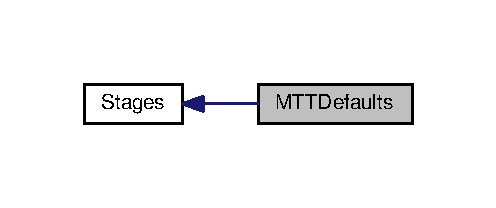
\includegraphics[width=238pt]{group__MTTDefaults}
\end{center}
\end{figure}
ordering 0 \hypertarget{group__MTTDefaults_DefaultMTTDefaults}{}\subsection{Default\-M\-T\-T\-Defaults}\label{group__MTTDefaults_DefaultMTTDefaults}

\begin{DoxyParams}{Parameters}
{\em trial} & Use when testing your M\-T\-T client setup; results that are generated and submitted to the database are marked as "trials" and are not included in normal reporting. \\
\hline
{\em scratch} & Specify the D\-I\-R\-E\-C\-T\-O\-R\-Y under which scratch files are to be stored \\
\hline
{\em description} & Provide a brief title/description to be included in the log for this test \\
\hline
{\em platform} & Name of the system under test \\
\hline
{\em organization} & Name of the organization running the test \\
\hline
{\em merge\-\_\-stdout\-\_\-stderr} & Merge stdout and stderr into one output stream \\
\hline
{\em stdout\-\_\-save\-\_\-lines} & Number of lines of stdout to save (-\/1 for unlimited) \\
\hline
{\em stderr\-\_\-save\-\_\-lines} & Number of lines of stderr to save (-\/1 for unlimited) \\
\hline
{\em executor} & Strategy to use\-: combinatorial or sequential executor \\
\hline
{\em time} & Record how long it takes to run each individual test \\
\hline
\end{DoxyParams}
